\section{Rule-based Heart Model Abstraction}
\label{ruleBasedHeartModelAbstraction}
Unlike system modeling in which there is only one concrete system, during environment modeling there are infinite number of environmental conditions that can be generalize by abstractions. In this section, we model the heart as the physiological environment for implantable pacemakers and try to cover different heart conditions and the closed-loop interactions between the heart and the pacemaker. Then using abstraction rules defined over physiological knowledge and principles for over-approximation we construct a series of heart model abstractions with different complexity and coverage. During the rule applications the merging of transition groups are documented thus can be used during model refinements.
\subsection{Electro-physiology (EP) Basics}
The heart generates periodic electrical impulses to control heart rates according to physiological needs. These impulses conduct through the heart, triggering coordinated muscle contractions and pump blood to the rest of the body. The underlying pattern and timing of these impulses determine the heart's rhythm and are the key to proper heart functions. Derangements in this rhythm are referred to as \emph{arrhythmia}, which impair the heart's ability to pump blood and compromise the patients' health. Arrhythmia are categorized into so-called \textsf{Tachycardia} and \textsf{Bradycardia}. Tachycardia features undesirable fast heart rate which results in inefficient blood pumping. Bradycardia features slow heart rate which results in insufficient blood supply. The electrical activities can be measured by inserting electrodes through the vein into the heart against the heart wall. Localized electrical activities can be measured, and the physicians can diagnose the heart conditions by delivering pacing sequence through the electrodes and observe the signal propagation. This procedure is referred to as Electrophysiological (EP) Testing  (\cite{josephson}) and the signals are referred to as electrograms (EGMs).

The implantable cardiac pacemakers are rhythm management devices designed to treat bradycardia. A typical dual chamber pacemaker has two leads inserted into the heart through the veins which can measure the local electrical activities of the right atrium and right ventricle, respectively. According to the timing between sensed impulses the pacemaker can deliver electrical pacing to the corresponding chamber to maintain proper heart rhythm.
\begin{figure}[!t]
\centering
		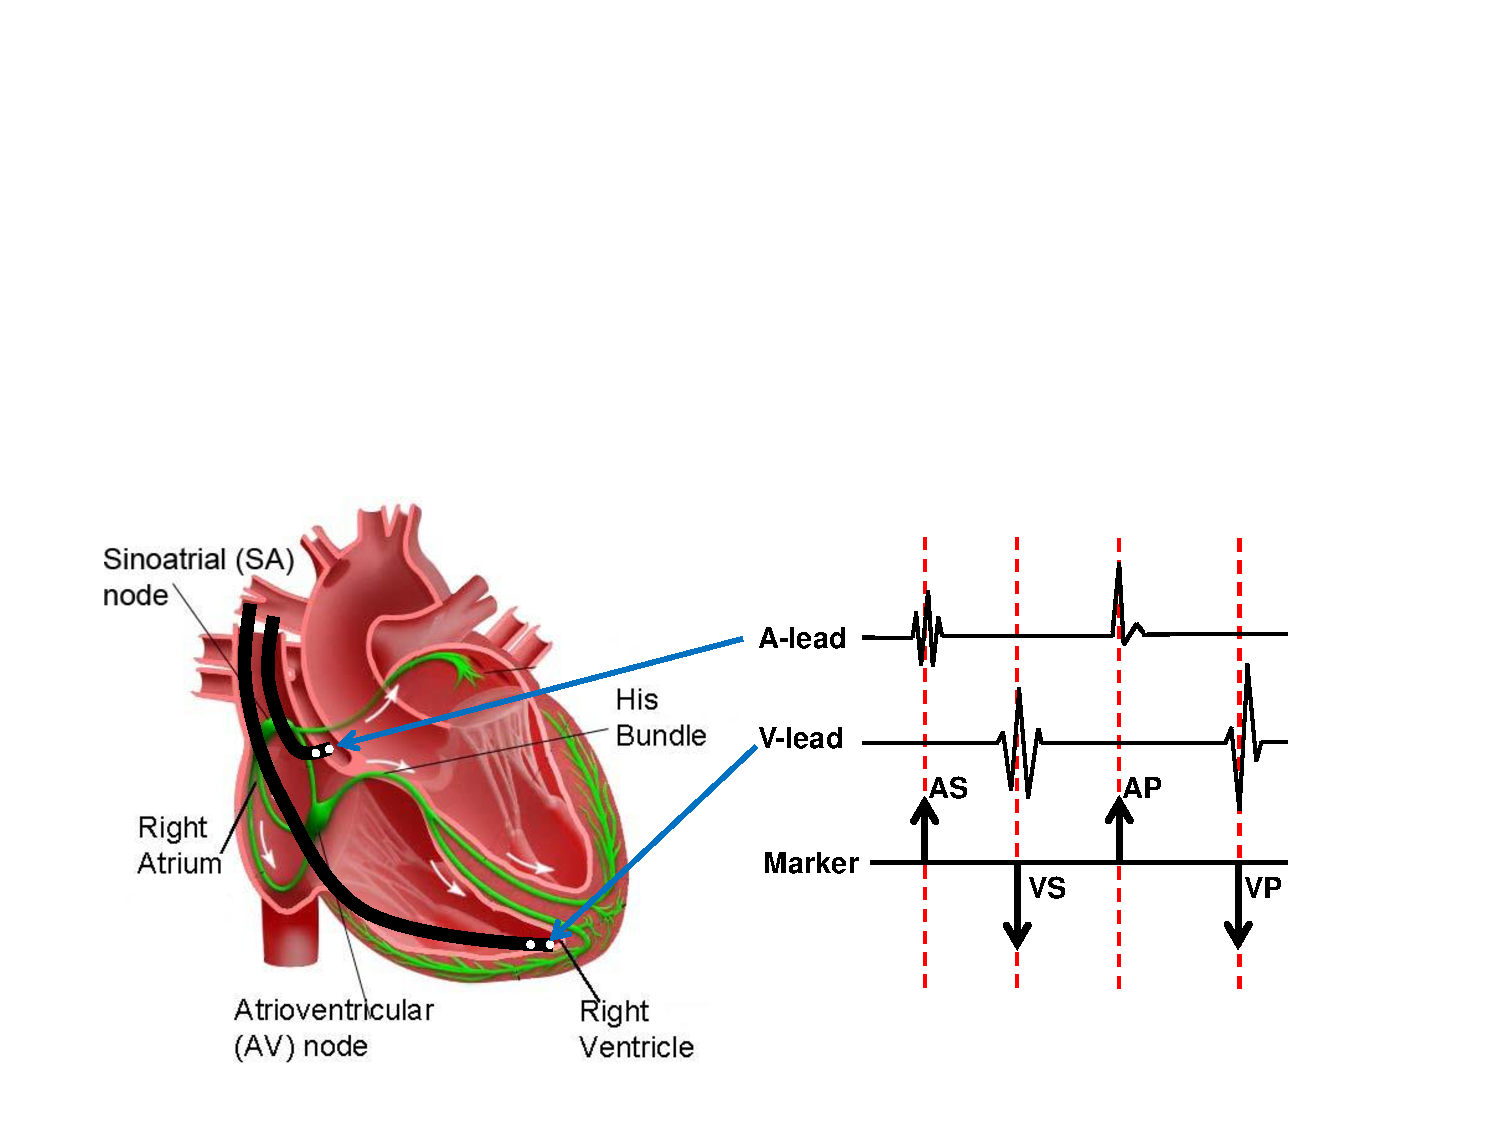
\includegraphics[width=0.7\textwidth]{figs/egm.pdf}
		
%\vspace{-10pt}
\caption{\small }
\label{fig:probes}
%\vspace{-15pt}
\end{figure} 
\subsection{The Virtual Heart Model (VHM)}
In \cite{VHM_proc} we developed a heart model structure based on ElectroPhysiology (EP). We use an extended timed-automata formulation (\cite{timed_automata}) to model the timing behaviors of heart tissue during each activation cycle. \figref{init}

 We refer the tissue model as \emph{Node automaton} and \figref{node_automata} shows the structure of a node automaton $i$. 3 states correspond to 3 timing periods of the action potential. From \textsf{Rest} state, the node can either self activate or activated by external stimuli (Act\_node) and go to \textsf{ERP} state. During \textsf{ERP} state the node does not respond to external stimuli (blocked). During \textsf{RRP} state, the node can still be activated and go to \textsf{ERP} state, however the ERP period and the conduction delay of the tissue are affected by the "earliness" of the activation arrived during the RRP period, which is tracked by a shared variable $C(i)$. The new ERP period is determined by a function over clock value $g(f(t))$ which mimic the beat-to-beat dynamics described in \cite{josephson}. 
\begin{figure}[!t]
		\centering
		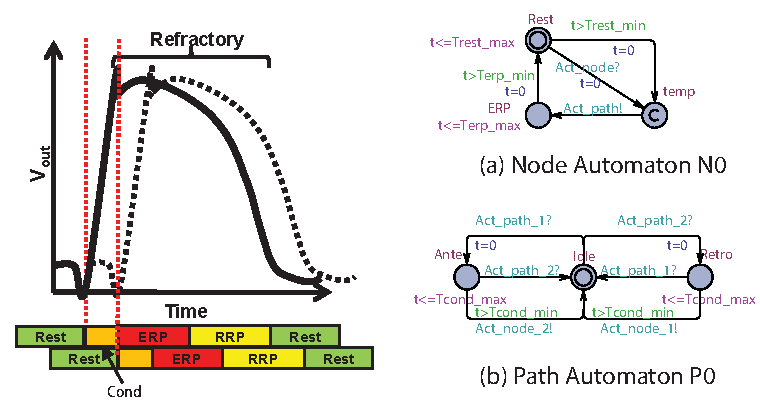
\includegraphics[width=0.8\textwidth]{figs/init_abs.pdf}
		%\vspace{-5pt}
		\caption{\small Heart Model Abstractions}
		  %\vspace{-15pt}
		\label{fig:init}
\end{figure}
The electrical conduction through the tissue between nodes are abstracted using \emph{path automata}. The path automata can be used to represent structural or topological (functional) electrical connections between nodes. \figref{path_automata} shows a path automaton connecting node a and b. The initial state of a path automaton is \emph{Idle}, which corresponds to no conduction. The states corresponding to the two conduction directions are named after the physiological terms: Antegrade (Ante) and Retrograde (Retro). These states can be intuitively described as forward and backward conductions. If \emph{Act\_path} event is received from one of the nodes connected to it, the a transition to \emph{Ante} or \emph{Retro} state correspondingly will occur in the path automaton. At the same time the clock invariant of the state is modified according to the shared variable \emph{C(a/b)}. This corresponds to the change of the conduction delay that is caused by the early activation. Similar to node automaton, the changing trend is extracted from clinical data. 

  %\begin{figure*}[!t]
%\centering
		%\subfigure [\small]{			
		%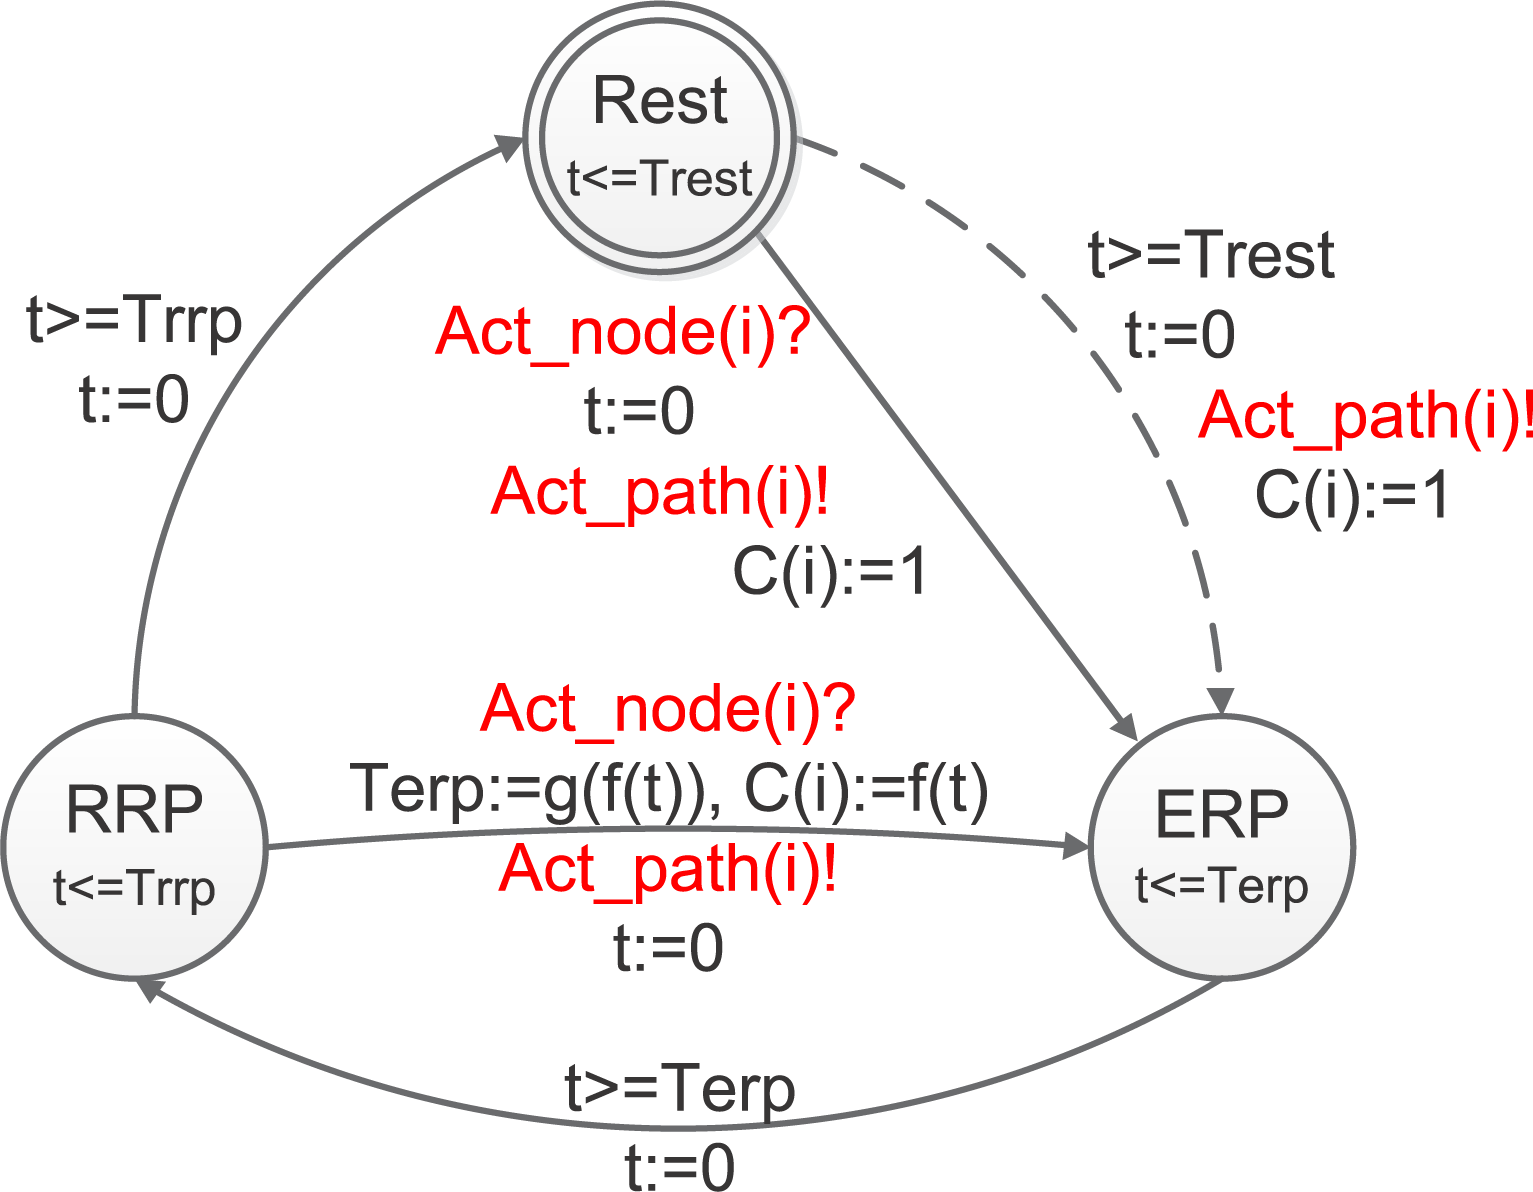
\includegraphics[width=0.35\textwidth]{figs/node_aut.png}
		%\label{fig:node_automata}
		%} 
%%	\hspace{.1in}%
		%\subfigure [\small] 
		%{
		%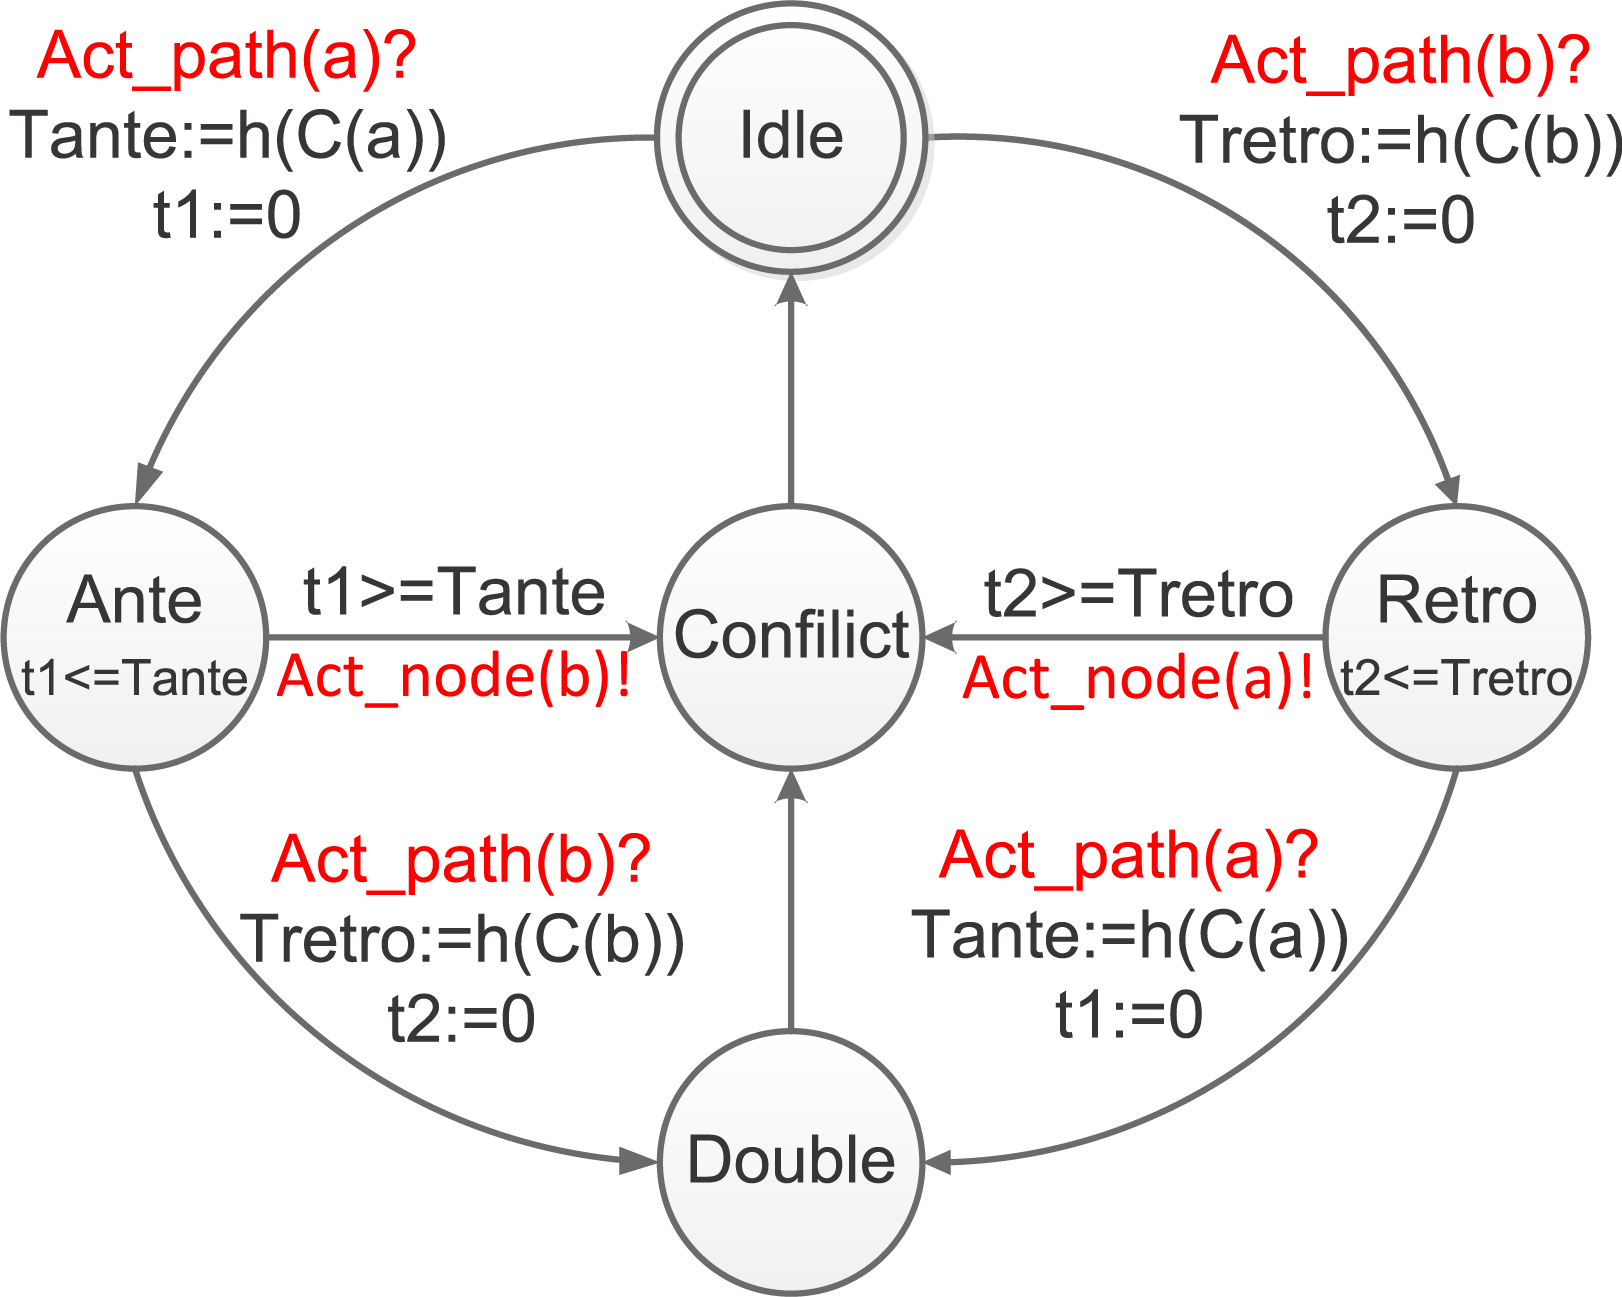
\includegraphics[width=0.35\textwidth]{figs/path_aut.png}
		%\label{fig:path_automata}
		%} 
		%\subfigure [\small] 
		%{
		%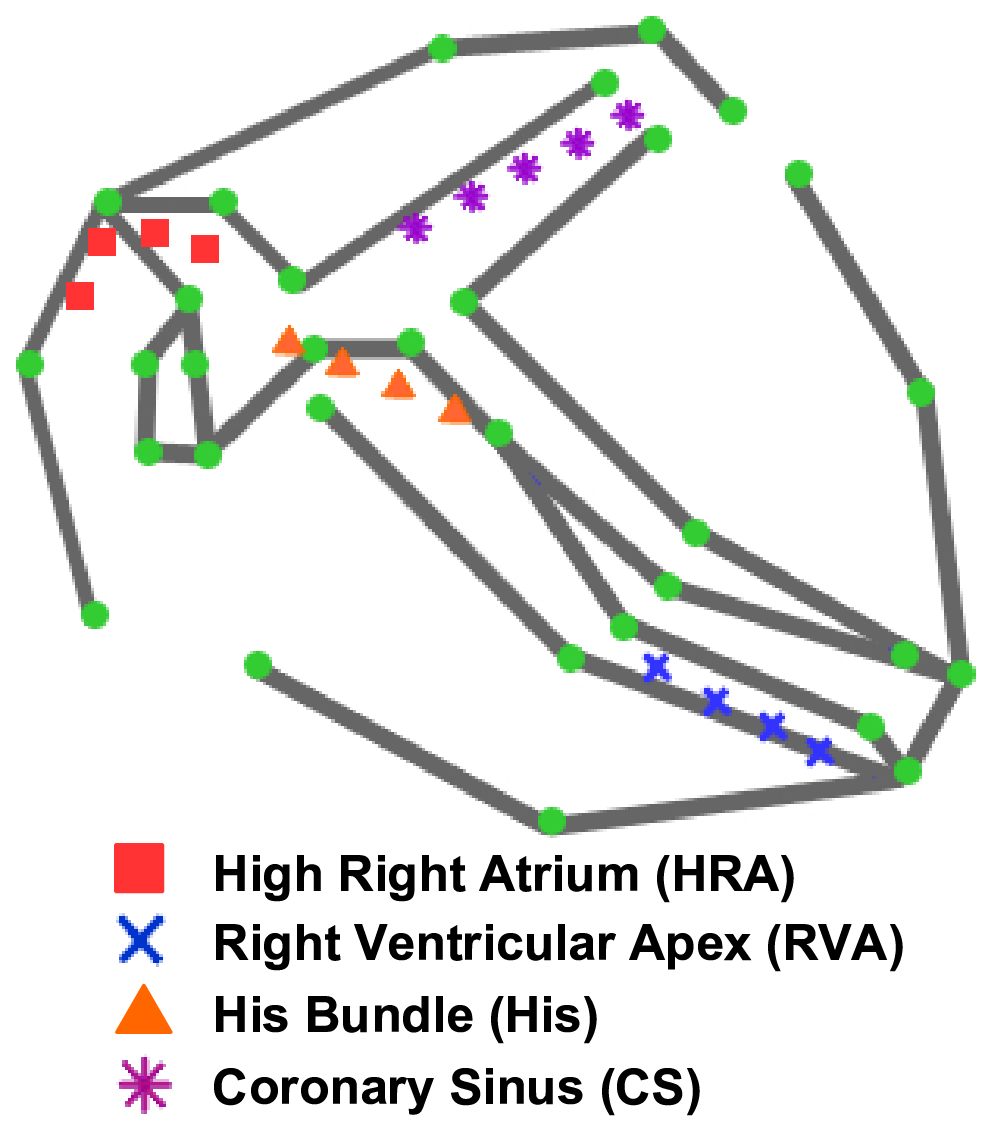
\includegraphics[width=0.2\textwidth]{figs/gen_setup.png}
		%\label{fig:general_setup}
		%} 
%\label{fig:h_automatas}
%%\vspace{-10pt}
%\caption{\small (a) Node automaton. Dotted transition is only valid for pacemaker tissue like SA node; (b) Path automaton; (c) Model of the electrical conduction system of the heart using a network of node \& path automata ~\cite{VHM_proc}.}
%%\vspace{-15pt}
%\end{figure*} 
\begin{figure}[!t]
		\centering
		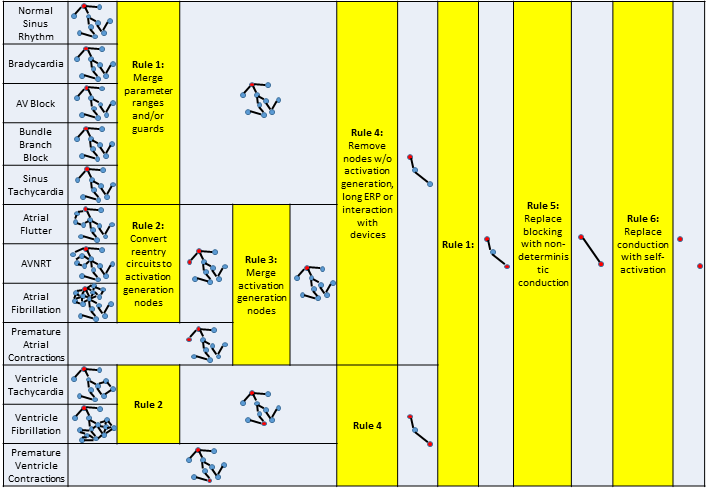
\includegraphics[width=0.9\textwidth]{figs/rule.png}
		%\vspace{-5pt}
		\caption{\small Heart Model Abstractions}
		  %\vspace{-15pt}
		\label{fig:abs}
\end{figure}


For a heart model $H$ with $n$ nodes and $m$ paths, the node automata are denoted as $N_i, i\in[1,n]$ and path automata are denoted as $P_j,j\in[1,m]$
\subsection{Rule 1: Merge Parameter Ranges}
The node and path automata model the timing periods with different properties. The parameters of the node and path automata are the ranges of time in which the automata can stay in corresponding locations. The lower range is specified as a clock invariant and the upper range is specified as a guard. Rule 1 is usually applied to heart models with the same node and path topology. 
 $$para\_min'=min(para\_min1,para\_min2\cdots para\_minN)$$ 
$$para\_max'=max(para\_max1,para\_max2\cdots para\_maxN)$$

\subsection{Rule 2: Convert Reentry Circuits to Activation Nodes}
\begin{figure}[!h]
		\centering
		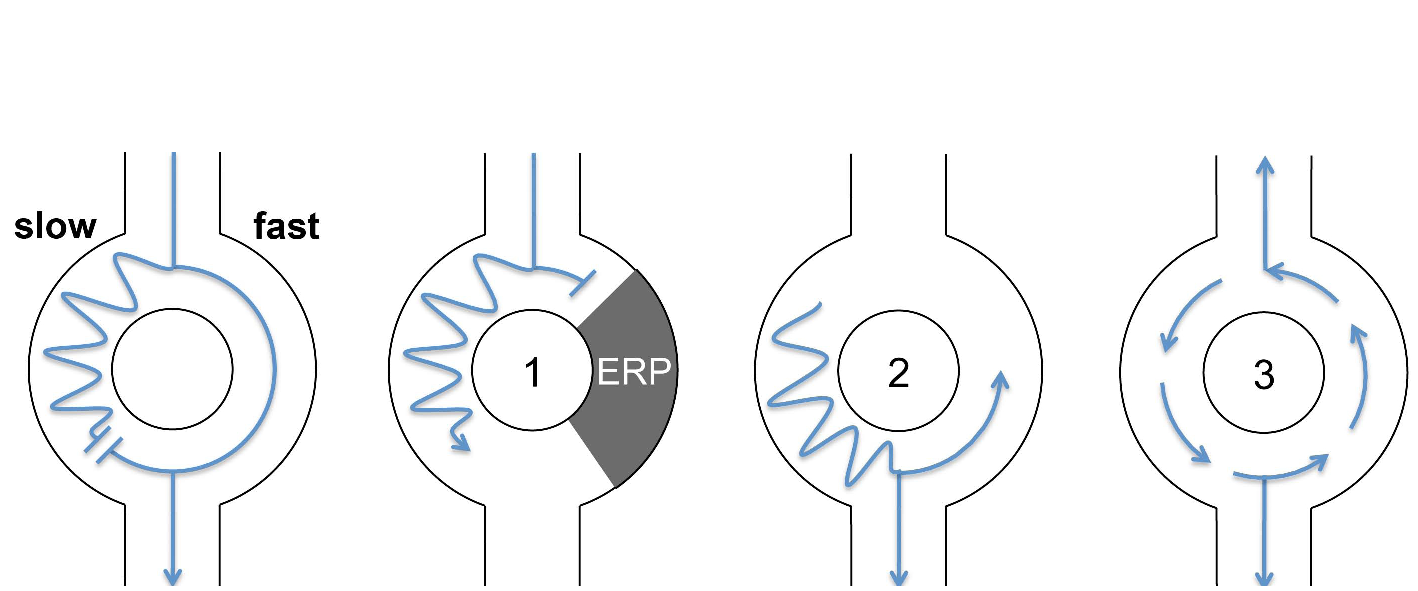
\includegraphics[width=0.6\textwidth]{figs/reentry.pdf}
		%\vspace{-5pt}
		\caption{\small Heart Model Abstractions}
		  %\vspace{-15pt}
		\label{fig:reentry}
\end{figure}
\subsection{Rule 3: Merge Activation Generation Nodes}
\subsection{Rule 4: Remove Structures that Do Not Affect Outputs}
\subsection{Rule 5: Replace Blocking With Non-deterministic Conduction}

\begin{figure}[!h]
		\centering
		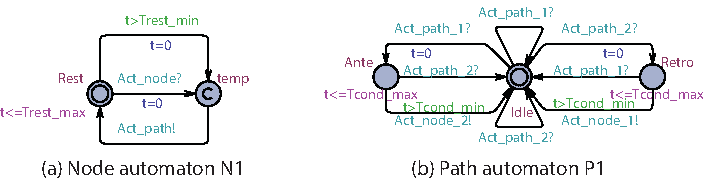
\includegraphics[width=0.9\textwidth]{figs/rule5.pdf}
		%\vspace{-5pt}
		\caption{\small Heart Model Abstractions}
		  %\vspace{-15pt}
		\label{fig:rule5}
\end{figure}
\subsection{Rule 6: Replace}

\begin{figure}[!h]
		\centering
		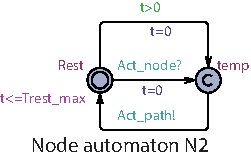
\includegraphics[width=0.3\textwidth]{figs/rule6.pdf}
		%\vspace{-5pt}
		\caption{\small Heart Model Abstractions}
		  %\vspace{-15pt}
		\label{fig:rule6}
\end{figure}
